\documentclass[tikz,border=10pt]{standalone}
\usepackage{tikz}
\usetikzlibrary{trees}

\begin{document}
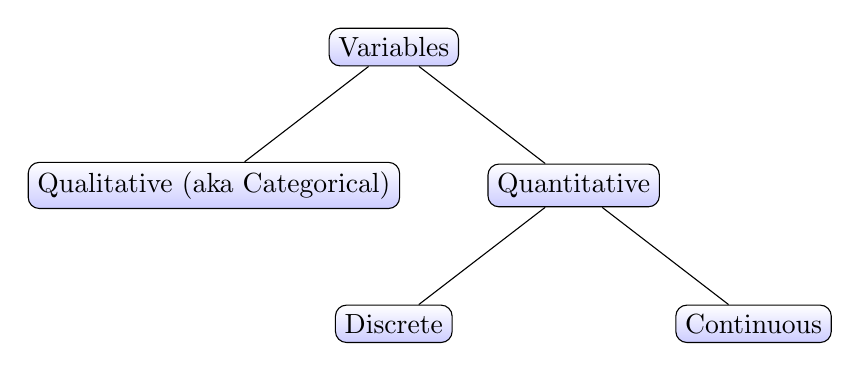
\begin{tikzpicture}
  [
    sibling distance=13em,
    level distance=5em,
    every node/.style = {shape=rectangle, rounded corners,
      draw, align=center,
      top color=white, bottom color=blue!20}
  ]
  \node {Variables}
    child { node {Qualitative (aka Categorical)} }
    child { node {Quantitative}
      child { node {Discrete} }
      child { node {Continuous} } };
\end{tikzpicture}
\end{document}
